%!TEX root = ../thesis.tex
%*******************************************************************************
%****************************** Second Chapter *********************************
%*******************************************************************************

\chapter{Results of Physical Properties Modification in Novel 2D materials \label{chap:5}}

\ifpdf
    \graphicspath{{Chapter5/Figs/Raster/}{Chapter5/Figs/PDF/}{Chapter5/Figs/}{Chapter5/Figs/Vector/}}
\else
    \graphicspath{{Chapter5/Figs/Vector/}{Chapter5/Figs/}}
\fi

\section{Number of layers and types of stackings}
\subsection[Few-layer of Calcium hydroxide]{Few-layer of Calcium hydroxide \footcite[This work is published in:][]{Aierken2015.porlandite}}
\subsection[Few-layer of pentasilicene]{Few-layer of pentasilicene \footcite[This work is published in:][]{Aierken2016.pentasilicene}}

\section{Mechanical strain}
\subsection[Variation of vibrational modes under strain in phosphorene]{Variation of vibrational modes under strain in phosphorene \footcite[This work is published in:][]{Aierken2015.thermalP}}

In \autoref{sec:pho_phos} we calculated the phonon dispersion of black and blue phosphorene, here we will discuss how the vibrational modes change with strain. In \autoref{fig:ire_phos} we revisit the phonon dispersion of phosphorene, here the $\Gamma$ point vibrational modes with their irreducible representations and their frequencies are given.

\begin{figure}[htbp]
\centering
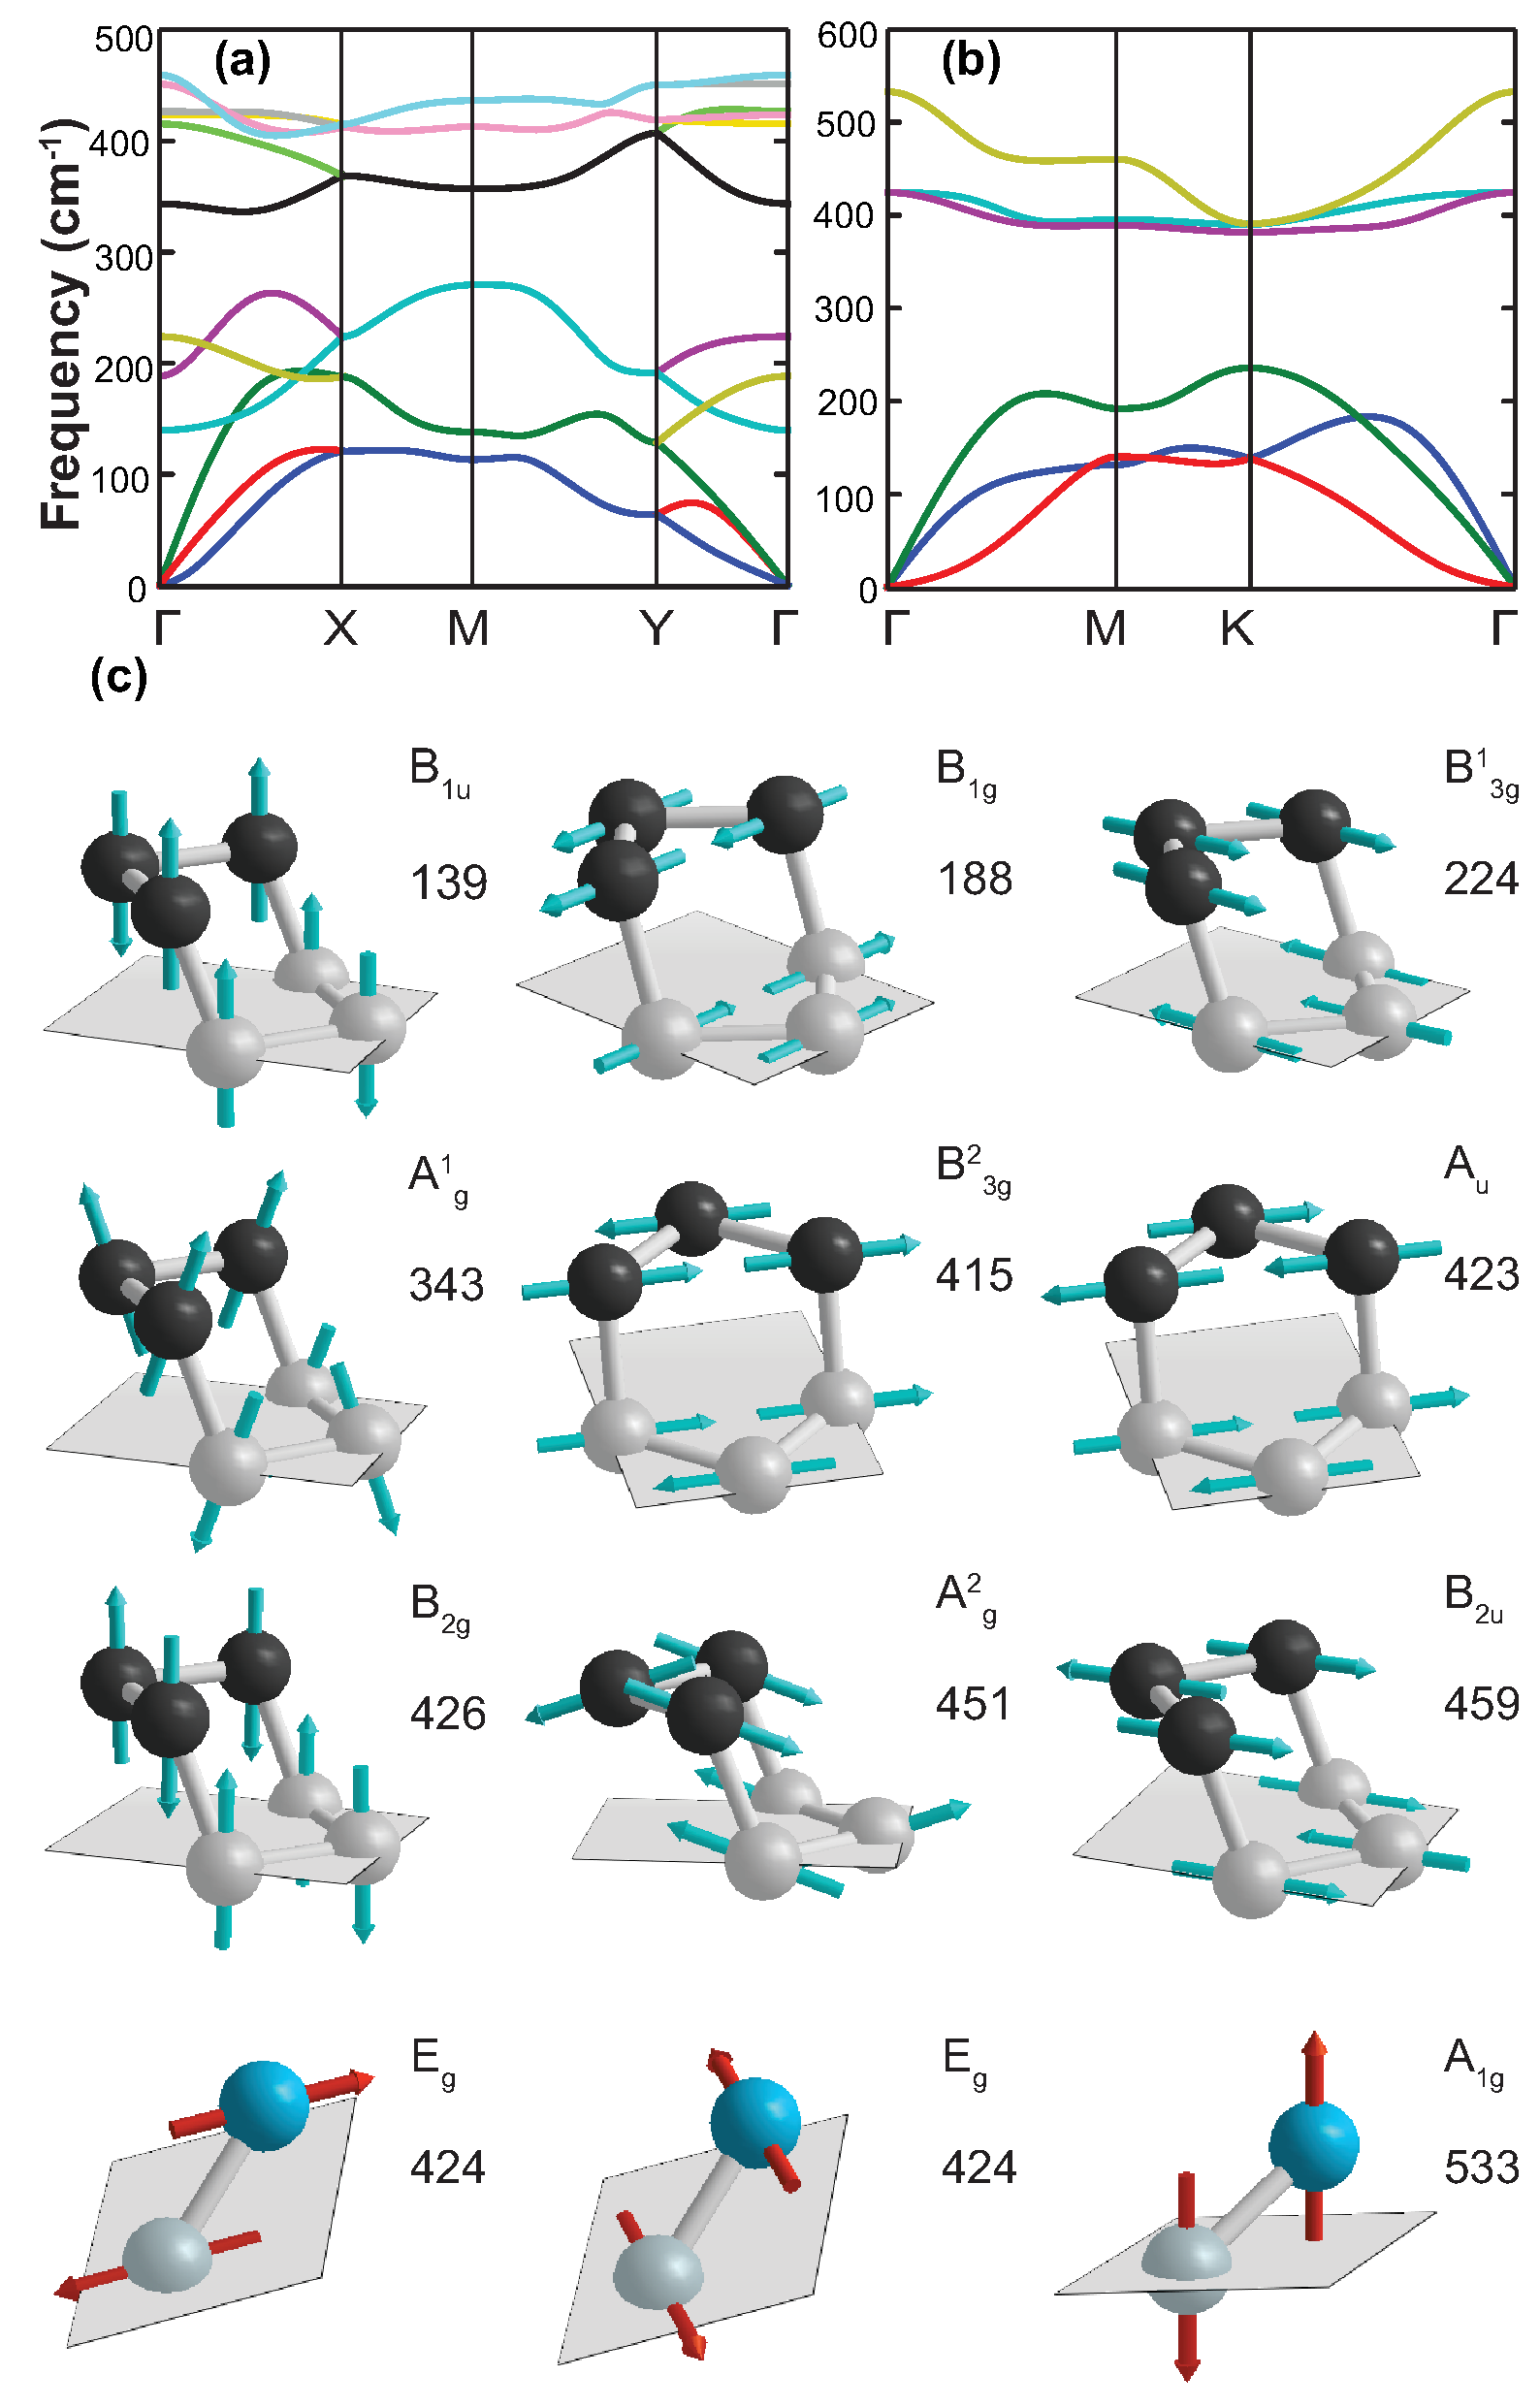
\includegraphics[width=0.8\linewidth]{phos_phon.eps}%
\caption{Calculated phonon dispersions for prinstine (a) black and (b) blue P. (c) Optical phonon modes together with their frequencies (in units of cm$^{-1}$) at the $\Gamma$ point and irreducible representations for black P and blue P. (c) Optical phonon modes together with their frequencies (in units of cm$^{-1}$) at the $\Gamma$ point and irreducible representations for black P and blue P.\label{fig:ire_phos}}
\end{figure}

\begin{figure}[htbp]
\centering
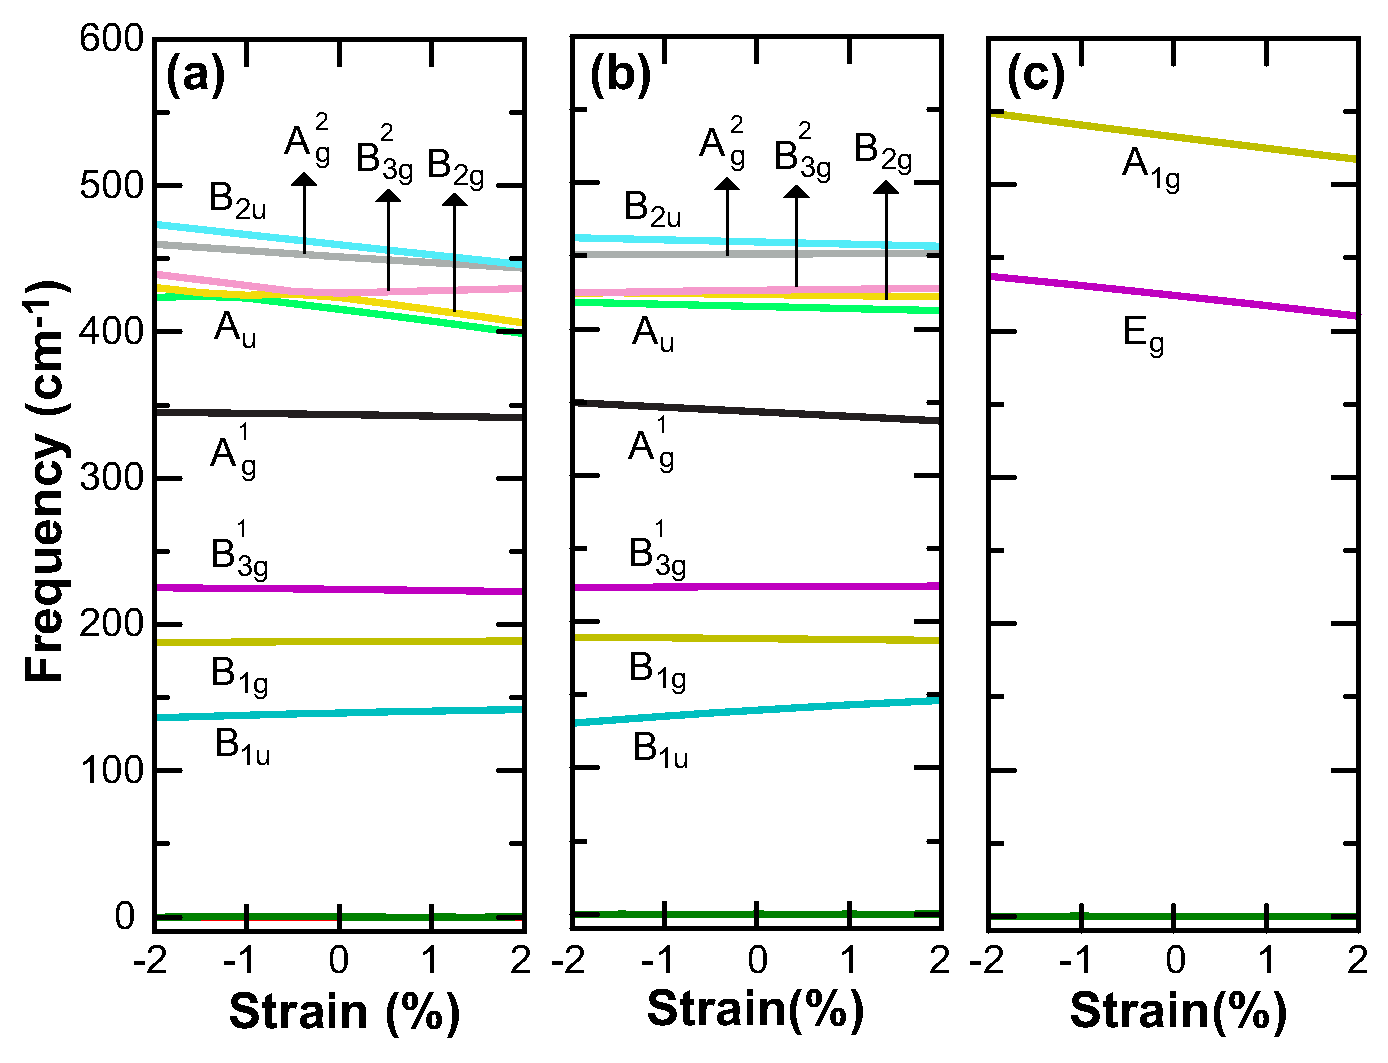
\includegraphics[width=0.8\linewidth]{strain_vib.eps}%
\caption{ (Color online) Variation of the $\Gamma$ frequencies with strain: (a) zigzag and (b) armchair direction of black P and (c) blue P.  \label{fig:shift_phos} }
\end{figure}

With the knowledge of the space group and its character table it is possible to assign vibrational modes to each band at the $\Gamma$-point. A table of all optical modes together with its frequency and irreducible representation for both structures is presented in \autoref{fig:ire_phos}(c) for the strainless structures. In \autoref{fig:shift_phos}, we show the variation of these optical phonons at the $\Gamma$ point under uniaxial strain. Our calculations agree well with the results of Ref.~\cite{phonon-blackP-1}. The frequency shift by strain can be directly detected using Raman spectroscopy. 
Depending on the atomic motion of the modes, the magnitude and type of strain, we find that the dependence of the phonon frequency can be different for each mode. Especially, the higher energy optical modes under uniaxial strain, applied along the zigzag direction, exhibit a much larger variation, see \autoref{fig:shift_phos}(a). B$^2_{3g}$ mode of black P has a different behavior under tensile and compressive strains along the zigzag direction. Applying a tensile (compressive) strain increases (decreases) the frequency of B$^2_{3g}$ mode. The frequency spacing between A$^2_{g}$ and B$_{2u}$ modes decreases when black P is stretched along both zigzag and armchair directions. While  the frequency of A$^2_{g}$ mode exhibits almost no variation under strain applied along the armchair direction,  it significantly varies under  strain applied along the zigzag direction.
Among the low lying optical modes (i.e., B$_{1u}$, B$_{1g}$ and B$^1_{3g}$), the B$_{1u}$ mode exhibits a larger variation with applied strain. 
E$_g$ and A$_{1g}$ modes of blue P always are red shifted when changing strain from compressive to tensile. Our results show that by measuring the frequency shift in the particular modes, it is possible to determine the
strain distribution in phosphorene.  

Our results show that the frequency shift observed in particular modes can be utilized to determine strain distribution in phosphorene.

\subsection[Carrier mobility enhancement in TiS$_3$ monolayer with strain]{Carrier mobility enhancement in TiS$_3$ monolayer with strain \footcite[This work is published in:][]{Aierken2016.mobility}}

%\subsection{Monolayer TiS$_3$}
%
%Bulk TiS$_3$ has a layered structure that makes it possible to exfoliate its monolayer. Indeed, such a process has been carried out by \citet{ADOM:ADOM201400043,ADMA:ADMA201405632} and results in the successful synthesis of a new type of 2D materials: monolayer TiS$_3$. The atomic structure of TiS$_3$ monolayer is shown in Fig.~\ref{structure}. The unit cell has a monoclinic crystal structure. The calculated lattice constants  are \textit{a} =  5.03 ~{\AA} and \textit{b} = 3.41~{\AA}, in good agreement with previous calculations \cite{Kang2015,Jin2015} and close to the experimental values for the bulk structure ($a$=4.958, $b$=3.401)\cite{Furuseth1975}. The monolayer is composed of connecting quasi-one-dimensional chains of TiS$_3$ triangular prisms extending along the \textit{b} direction, as shown in Fig.~\ref{structure}. One can spot a significant structural anisotropy in the system along the chain direction (green vector) and  the perpendicular direction (red vector).

\subsection{Carrier mobility}

\subsection[Magnetic properties modulation in penta-hexa-graphnene with strain]{Magnetic properties modulation in penta-hexa-graphnene with strain \footcite[This work is published in:][]{Aierken2016.magnetism}}

\begin{figure}[htbp]
\centering
\includegraphics[width=\linewidth]{FM_AFM.eps}%   
\caption{AFM to FM transition of monolayer ph-graphene under strain. \label{transition}}
\end{figure}

Strain is an effective way to modulate the electronic properties of materials. \textcolor{red}{There are different ways to induce strain on 2D materials. \citet{Roldan2015} gave a comprehensive review on the strain engineering on 2D system both from experimental and theoretical view. }Here, we apply biaxial strain to our structure and monitor how the total energy of the different magnetic phases change, see \autoref{transition}. We find that an AFM to FM transition occurs for both compressive and tensile strains of approximately 6\% and 8\%, respectively. Therefore, strained structures of this kind can give a FM ground state, which is more beneficial for applications. The variation of the band gap under strain is plotted in \autoref{bandgap}. Both the FM and the AFM band gap has a similar qualitative behavior with a small quantitative difference between the two magnetic phases. The tensile strain decreases the band gap monotonically up to 10\%, while the compressive strain gives a non-monotonic behavior due to band crossings. From -5\% to 10\% strain, CBM and VBM are located at the $\Gamma$ and K high symmetric k-points, respectively. While two transitions of the location of the VBM happen below -5\% strain. First, it is shifted to the $\Gamma$ k-point from the second highest valence band around -8\%, and then shifted to the $\Sigma$ k-path between the $\Gamma$ and M k-points at -9\%.

\begin{figure}[htbp]
\centering
\includegraphics[width=\linewidth]{FM_AFM_Eg.eps}%   
\caption{ (Color online) Band gap variation of AFM and FM monolayer ph-graphene under strain. \label{bandgap}}
\end{figure}
\begin{figure}[htbp]
\centering
\includegraphics[width=\linewidth]{AFM_AFM_barrier.eps}%   
\caption{ (Color online) AFM to FM transition through spin-flip in monolayer ph-graphene. \label{spinflip} }
\end{figure}

As a final property of the two different magnetic ground states, we study the energy barrier for the transition from the FM to AFM state through spin flipping. This calculation is realized by constraining the magnetic moment through a penalty contribution to the total energy in VASP, and rotate one of the moments stepwise through 180$^{\circ}$.  In this way an energy profile from FM to AFM can be obtained (see \autoref{spinflip}). The rotation of the magnetic moment was carried along two different planes, one along the zigzag direction and the other along armchair direction, but the difference of the energy profile is negligible. Without strain, there is almost no energy barrier for the transition from the FM to AFM state. However, if the structure is under a 9\% tensile strain, in which case the FM state is the ground state, an energy barrier of about 13 meV per magnetic atom arises to return to the AFM state. This is much larger as one consider the energy barrier from the AFM to the FM under the same strain, which is about 3.3 meV per magnetic atom. \textcolor{red}{This calculation is performed with the aim to study the stability of each magnetic state, and the possibility to form paramagnetic state even without thermal mothion. We found both magnetic state is stable, and there is no tendency to form non-collinear magnetic moment orientation, and possibility of paramagnetic formation is small.}

We discovered a strain-driven magnetic ground state transition from AFM to FM around  6\% compressive strain and 8\% tensile strain. An energy profile with different angles between two local magnetic moments is calculated to study the energy barrier for the transition between FM and AFM. While an energy barrier of about 13 meV/(magnetic atom) protecting the AFM ground state in the pristine case; it is protecting the FM ground state when the system is under 9\% tensile strain.  

\section{Adatom adsorption}
\subsection[Nitrogen edge-decorated graphene nanoribbon]{Nitrogen edge-decorated graphene nanoribbon \footcite[This work will be published as:][]{Aierken2017.GNR}}

\section{Heterostructures}
\subsection[Electrical transport in 1T/2H/1T MoS2 lateral heterostructure]{Electrical transport in 1T/2H/1T MoS2 lateral heterostructure \footcite[This work is submitted as:][]{Aierken2017.transport}}
\subsection[Li storage and diffusion in MXenes/graphene vertial heterostructure]{Li storage and diffusion in MXenes/graphene vertial heterostructure \footcite[This work will be published as:][]{Aierken2017.battery}}

\section{Defect induction}
\subsection[Faceted blue phosphorene nanotube formed by line defects]{Faceted blue phosphorene nanotube formed by line defects \footcite[This work is published in:][]{Aierken2015.nanotubes}}
\subsection[Electronic structure of penta-hexa defects in graphene]{Electronic structure of penta-hexa defects in graphene \footcite[This work is published in:][]{Aierken2016.magnetism}}